\section{\bfseries Analiza sistema}

Osnovna svrha sistema je da omogući korisnicima aplikacije da lako i efikasno pronađu prevoz od jednog odredišta do drugog. Aplikacija unutar ovog projekta ograničiće se na gradski i međugradski prevoz unutar jedne države, tj. neće pružati usluge međunarodne vožnje. Aplikacija će, pored gorepomenute usluge, pružati mogućnost korisnicima da se lako informišu, prijave i obuče za vozače koji će ubuduće drugim korisnicima pružati usluge i pritom biti plaćeni za svoj rad. Naša CarGo aplikacija kao primarni zadatak ima da pruži bezbednu vožnju i vozaču i putnicima, što omogućavaju razne mere predostrožnosti, poput redovnih provera vozača u vidu testova ličnosti, snalaženja u saobraćaju i njihovog poznavanja zakona, redovne mehaničke provere vozila, mogućnost ocenjivanja vozača, vozila a i putnika, i blokada naloga u slučaju nezadovoljavajućih rezultata. Dodatnu zaštitu putnika i vozača pružaju sigurnosne kamere unutar i van vozila, koje se mogu iskoristiti za rešavanje mogućih sporova. Aplikacija takođe obezbeđuje visoku količinu transparentnosti u vidu unapred poznate cene prevoza. Na kraju, cilj aplikacije je da obezbedi da i vozač i putnici budu zadovoljni i da je koriste i ubuduće.
     
\subsection{\bfseries Dijagram konteksta}

\quad Na slici \ref{fig:CarGoContextDiagram} prikazani su dijagram konteksta i akteri, a na slici \ref{fig:dtp1} je dat dijagram toka podataka nivoa jedan.
\paragraph{Registrovanje korisnika:}
    Da bi korisnik mogao da se prijavi prvo mora da se registruje. Registraciju obavlja sam i dobija odgovor na kraju da li je uspe\v sno registrovan ili ne.
\paragraph{Login korisnika:}
    Da bi korisnik mogao da zatra\v zi vo\v znju mora biti prijavljen. On to radi samostalno i kao odgovor dobija da li se uspe\v sno prijavio.
\paragraph{Rad sa voza\v cima:}
    Uslov da bi voza\v c mogao da vozi korisnike je da on bude registrovan. Proces registracije obavlja uspomo\' c HR slu\v zbe. Tako\dj e voza\v c, ukoliko nije pogodan, mo\v ze biti obrisan iz sistema i samim tim će mu biti zabranjeno da dalje prevozi korisnike. Taj posao obavlja HR. Ukoliko novoregistrovani voza\v c nema svoje vozilo, HR pravi zahtev \v sefu voznog parka i daje na kori\v sćenje voza\v cu.
\paragraph{Login voza\v ca:}
    Kako bi mogao da prevozi korisnike, voza\v c prvo mora da se prijavi. On to radi samostalno i kao odgovor dobija da li se uspe\v sno prijavio.
\paragraph{Vo\v znja:}
    Korisnik napravi zahtev za vo\v znju, slobodan voza\v c prihvati. Voza\v c do\dj e na dogovorenu lokaciju i preveze korisnika na \v zeljeno mesto. Korisnik na jedan od dva ponu\dj ena na\v cina plati vo\v znju i opciono oceni voza\v ca.
\paragraph{Nabavka vozila:}
    U sistemu postoje dve vrste voza\v ca. Voza\v ci koji imaju svoj automobil i oni koji dobijaju automobil na kori\v s\' cenje prilikom registracije. Da se ne bi desilo da nema slobodnih automobila za novoregistrovanog voza\v ca, \v sef voznog parka obavlja nabavku novih automobila.

\begin{figure}[H]
\begin{center}
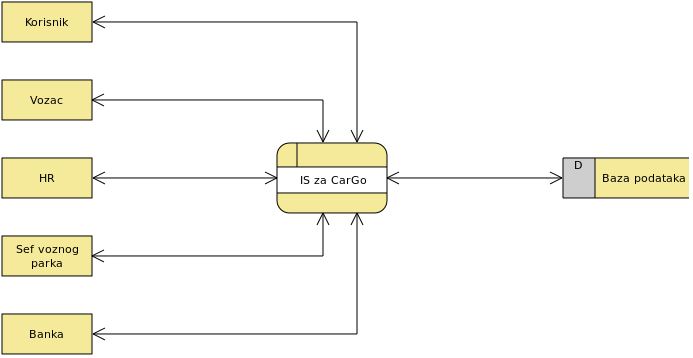
\includegraphics[width=\textwidth]{CarGoContextDiagram.png}
\end{center}
    \caption{Dijagram konteksta infomacionog sistema.}
\label{fig:CarGoContextDiagram}
\end{figure}

\begin{figure}[H]
\begin{center}
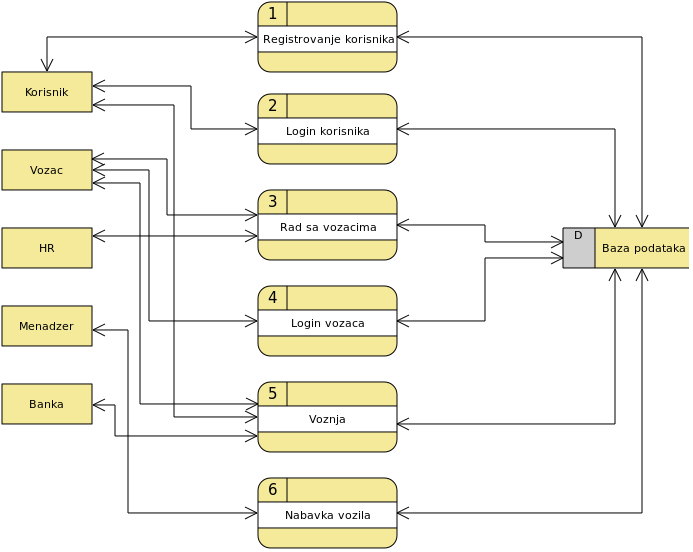
\includegraphics[width=\textwidth]{ISzaCarGo.png}
\end{center}
    \caption{Dijagram toka podataka nivoa 1.}
\label{fig:dtp1}
\end{figure}

\subsection{\bfseries Akteri}
\begin{itemize}
    \item Korisnici ovog sistema su svi oni kojima je potreban transport od jednog odredišta do drugog. Možemo ih podeliti na fizička i pravna lica. 
    \begin{itemize}
        \item Fizička lica - osobe koje usluge ovog sistema koriste preko svojih računa
        \item Pravna lica - osobe koje usluge ovog sistema koriste preko računa firme u kojoj rade
    \end{itemize}
    \item Vozači su ljudi kojima ovaj informacioni sistem posreduje kako bi izvršavali usluge korisnicima kojima je potreban prevoz. Vozači većinski koriste svoje automobile za prevoz.
    \item Banka je posrednik u transakciji između korisnika i vozača nakon izvršene usluge.
    \item Dobavljači vozila su grupa ljudi koja se bavi nabavkom dela vozila koja se koristi za prevoz korisnika
    \item HR tim je grupa ljudi koja odlučuje ko je podoban da bude vozač, odnosno ko je bezbedan po korisnike sistema i ima dozvolu za vozilo kojim upravlja. Ukoliko vozač nema svoje vozilo ovaj tim je dužan da o tome obavesti šefa voznog parka.
     \item Šef voznog parka je osoba koja je sastavlja porudžbine o broju vozila neophodnih vozačima koju šalje dobavljačima.
\end{itemize}